\documentclass[twocolumn,preprintnumbers,superscriptaddress,amsmath,amssymb,floatfix]{revtex4-1}

%superscriptaddress

\usepackage{graphicx}% Include figure files
\usepackage{dcolumn}% Align table columns on decimal point
\usepackage{bm}% bold math
\usepackage{color}
\usepackage{epstopdf}
\usepackage{multirow}
\usepackage{float}
\restylefloat{table}


\begin{document}

\preprint{}

\title{Digital Signal Pulse Processing}

\author{J.A.Brown}
\affiliation{Department of Nuclear Engineering, University of California, Berkeley, California 94720, USA}
\affiliation{Lawrence Lawrence Livermore National Laboratory, Berkeley, California 94720, USA}

\author{A.P. Priest}
\affiliation{Lab Partner}

%\date{\today}% It is always \today, today.
             
\begin{abstract}
\noindent This experiment explored the benefits and parameter space of digital signal processing applied to $\gamma$ radiation detection. A high-purity germanium (HPGe) detector was coupled simultaneously to both a digital and analog data-acquisition system. The parameters were optimized for both configurations. For the analog system, the shaping time was corrected to find a minimum full width half maximum (FWHM) of a 59.54 KeV $^{241}Am$ $\gamma$ line and the resultant resolution for a number of energies. For the digital system, the convolution developed by Jordanov \cite{jordanov_1} as a trapezoidal shaping filter was interpreted using linear algebra methods, the shaping time and gap time were optimized using a combination of $\gamma$ lines from  $^{241}Am$ and $^{60}Co$, the energy dependent resolution was measured, and the fano factor was calculated from the resultant spectra.
\end{abstract}

%\pacs{XX}
%   24.10.-i - Nuclear reaction models and methods
% 24.75.+i	General properties of fission
% 24.87.+y Nuclear reactions, surrogate reactions
% 25.55.-e <sup>3</sup>H-, <sup>3</sup>He-, and <sup>4</sup>He-induced reactions
% 25.85.Ge	Charged-particle-induced fission
% 29.30.Kv Gamma-ray spectroscopy, nuclear physics
% 21.10.-k Properties of nuclei; nuclear energy levels
% 27.90.+b A>= 220
%23.20.Lv	? transitions and level energies
%25.20.Dc	Photon absorption and scattering

\maketitle

\section{Introduction}
\label{intro}
The advent of new fast digitization methods invoked a revolution in the field of radiation detection. Digital acquisition techniques allow for a single data acquisition system to be employed with an array of detection modalities, software being the only change needed. Digital pulse processing methods also allow flexibility in post processing not possible with analog equipment. The use of analog equipment involves a fundamental loss of information about the signal itself, only recording chosen characteristics. This lab investigates these digital methods and contrasts them with older techniques. It does this using high purity germanium detectors and calibration sources exploring the characteristics of the germanium detector and the acquisition system in concert. The apparatus used and its configuration are detailed in Sec. ~\ref{exp}. A description of the pulse processing method developed and implemented are detailed in Sec.~\ref{methods}. Finally the experimental data are presented and discussed in Sec ~\ref{data}. 
  

\section{Methods}
\label{methods}
All of the data analysis for this lab was done in either CERN's root data analysis package \cite{root} or Anaconda's python package\cite{python}. For the filtering, Jordanov develops a trapezoidal filter as a superposition of two step functions and two ramp functions. Convolving this with an exponentially decaying signal returns a pole zero corrected trapezoidal shape.\cite{jordanov_1} The step height is equal to $\tau$ the correction factor to account for the exponential decay of the pre-amplifier signal. The width of the first step function is the peaking and gap time. The second step  is inverted with width equal to just the peaking time. Both of the ramp function widths are determined by the peaking time and have unit slope. The first ramp starts at 0 and has positive slope.  The second begins at the peaking plus gap time and has negative slope. Figure ~\ref{filter} shows a representative construction used for the analysis. The convolution of this and a pulse can be interpreted as a matrix product as illustrated by the following discussion. The $M_{th}$ element of the discrete convolution using summation notation is given by:

\begin{equation}
\label{conv_element}
(P*f)(t)_m = P_j(m) \cdot f_j(t-m)
\end{equation}

Where $P_j(t)$, $f_j(t)$ is $j_{th}$ component the exponential pulse and convolution function respectively. If a matrix of the form:  

\begin{equation}
\label{cond}
 F_{ik} =
  \begin{cases} 
      \hfill f_{j=k-i} \hfill & \text{ if $0 \leq k-i \leq j_{max}$} \\
      \hfill 0 \hfill & \text{ otherwise} \\
  \end{cases}
\end{equation}

\noindent with dimension equal to $ j_{max} \times j_{max} $ is constructed from the convolution function, then a column k is equivalent to $f(k-t)$. The $M_{th}$ element of the product of the original discretized pulse, $P(t)$, and this matrix has the form, again using summation notation:

\begin{equation}
\label{conv}
(P \cdot F)_{m} = P_{j} \cdot F_{jm}
\end{equation}

\noindent which is equivalent to the above expression for the convolution. If instead $P(t)$ is an array of pulses the matrix product becomes: 

\begin{equation}
\label{conv_full}
(P \cdot F)_{nm} = P_{nj} \cdot F_{jm}
\end{equation}

\noindent which allows the processing of multiple pulses with one line of code. To test the filter, an exponential decay signal with a known time constant was generated and the result of the matrix product was inspected to insure that the result was trapezoidal and that the signal returned to zero after the filter had fully passed over the rise of the exponential. This is illustrated in Figure ~\ref{filter_func}.



\begin{figure}
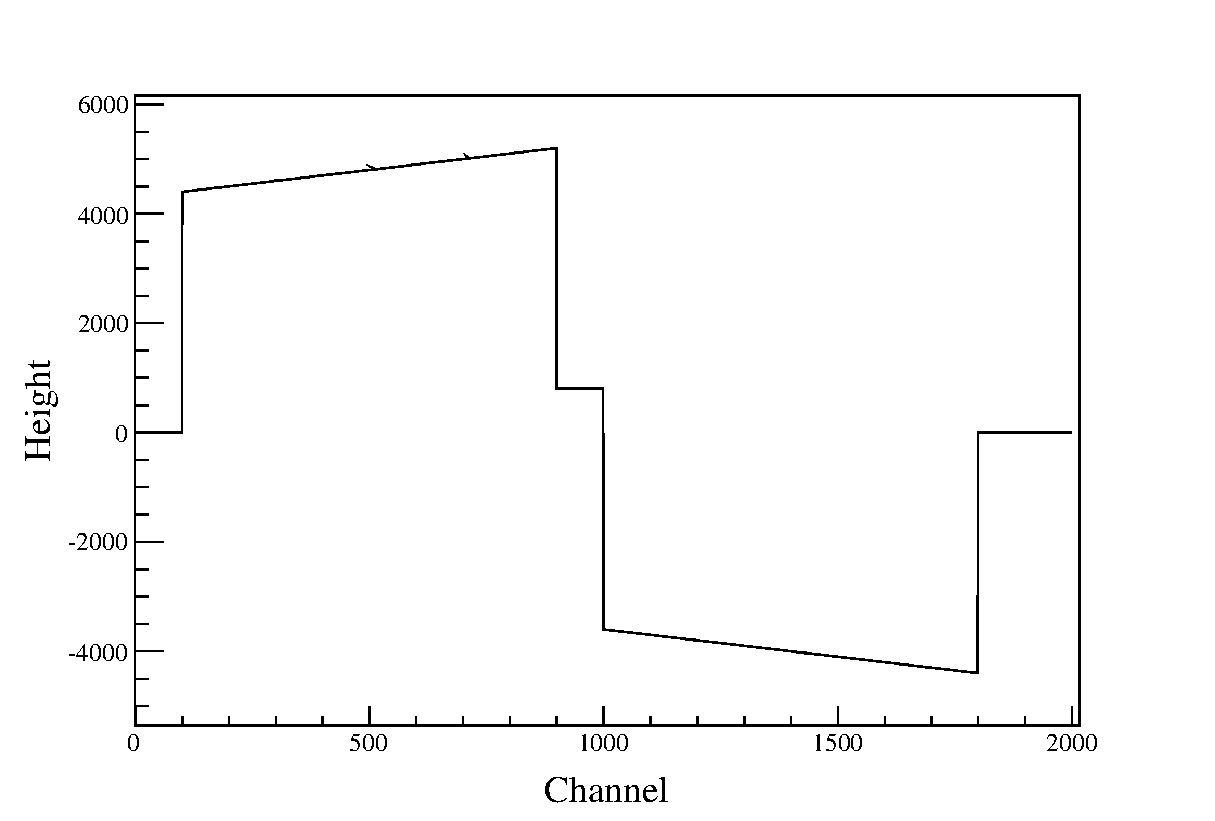
\includegraphics[width=0.47\textwidth]{filter.eps}
\caption{A trapezoidal filter with a peaking time of $8\mu S$ a gap time of $1 \mu s$ and $\tau$ equal to $44\mu s$ 
\label{filter}}
\end{figure}

\begin{figure}
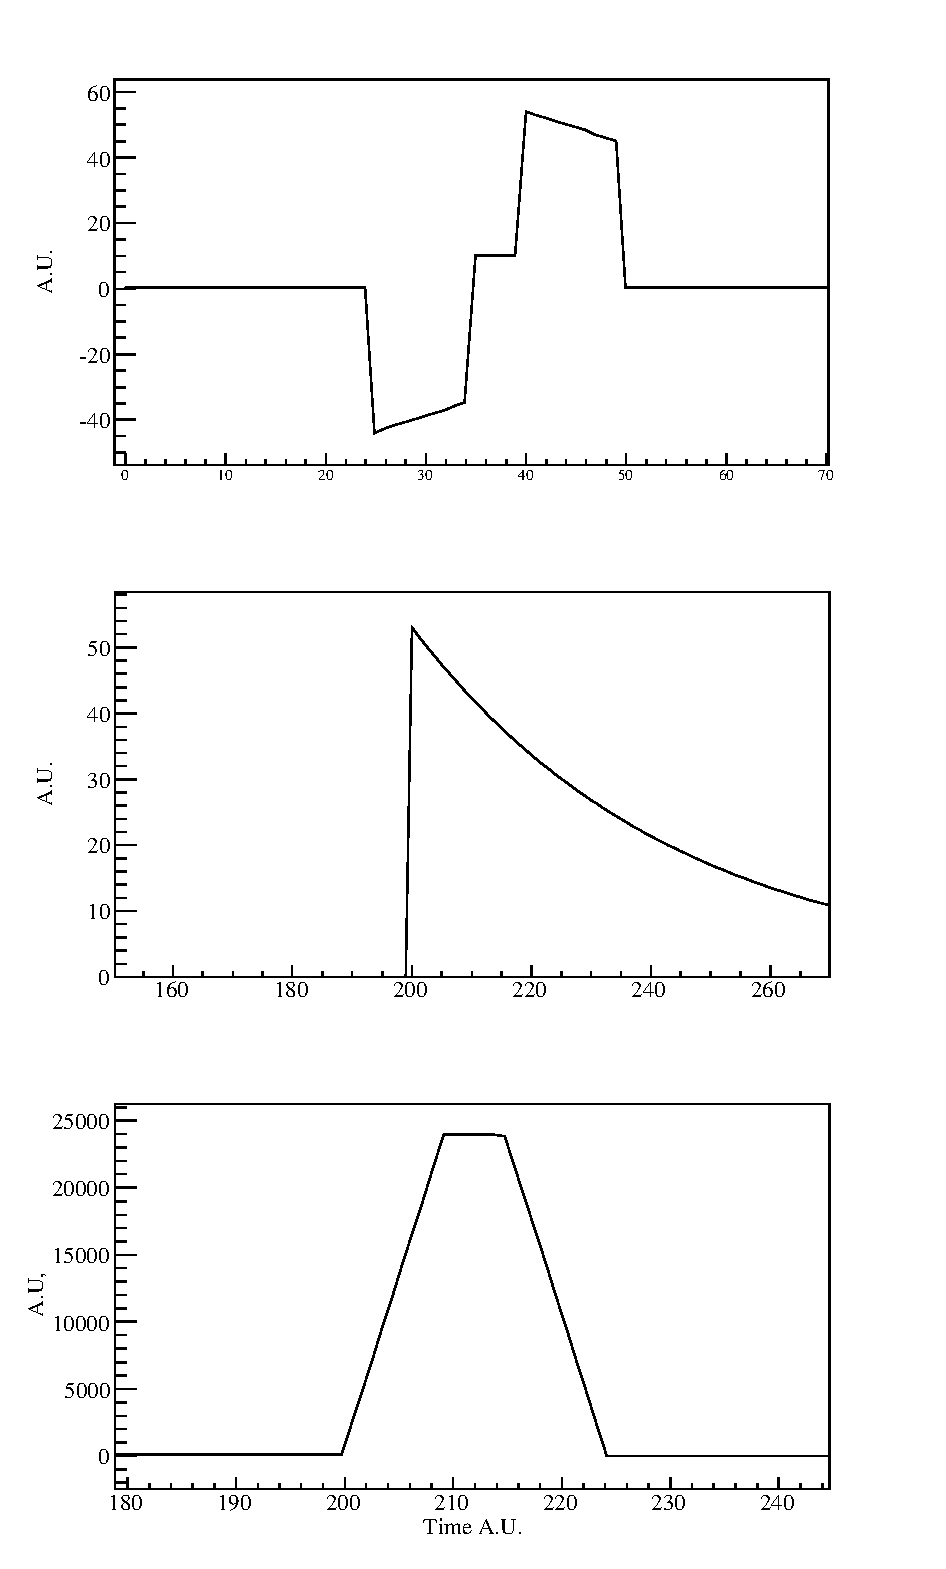
\includegraphics[width=0.5\textwidth]{filter_function_example.eps}
\caption{A projection of a row of the filter matrix (top) An exponential used as test input (middle) The resulting trapezoid (Bottom) \label{filter_func}}
\end{figure}

\section{Experimental Configuration}
\label{exp}
A Ortec (model) HPGe detector biased to $-3500 V$ was attached to two data acquisition systems. The first was an analog detection system that consisted of a shaping amplifier, using the raw output of the pre-amp for an input, coupled to a PCI based analog to digital converter.  The second detection system employed a struck SIS3302 analog to digital converter. The SIS3302 is a VME based waveform digitizer capable of collecting $100Ms/S$. Data were collected using this clock speed. The raw output from the preamplifier was used as an input to the system. The Struck module was managed by a controller card coupled to a software package developed by Struck via usb. The SIS3302 employs A field programmable gate array (FPGA) which is configurable through this software. It allows a fast and slow filter to work in coincidence on the raw input signals for detection of events and preliminary shaping to ensure data being taken includes signals of interest. This was first coupled to a  tail pulser to explore the configuration options available in the struck software. Data were then taken with the HPGe detector. For both acquisition systems $^{241}Am$ and $^{60}Co$ calibration sources were used to provide well known sources of $\gamma$ radiation. The distances of the sources were selected to ensure event rates of less than $1kHz$ making pile up events a negligible overall contribution. The full scale voltage range of the digitizer was determined to be $\pm 2.5$ V. The fast filter threshold values were set to insure both that the signals from the 59.5 Kev $\gamma$ were included in the data stream, and that the system did not trigger on noise. Trace lengths were selected to be 4000 samples, symmetric about the event, so that total integration times of up to 20 $\mu$S were possible.

\section{Results and Discussion}
\label{data}

\begin{figure}
\includegraphics[width=.5\textwidth]{peak_fit.eps}
\caption{A representative peak fit from the scipy fitting routine. The solid black line is the data, the dotted black line is fit function with minimized parameters, and the dashed line represents the residuals. 
\label{peak_fit}}
\end{figure}







To evaluate the gross behavior, both the gap time and peaking time were modified without calibrating to evaluate the spectral dependence on these parameters. The peak position is relatively independent of the gap time, but the height and shape do vary as characterized in following analysis. All the characteristics of the spectrum change with a change in peaking time. The peak location varies in the same direction as a change in peaking time. The other changes are explored in the following analysis. To determine the appropriate filter parameters for use with the germanium detector, data were analyzed for a number of parameters. First, a gap time of $1\mu S$ was selected and the peaking time was varied in $1\mu s$ increments from $2\mu s$ to $16\mu s$. For each chosen parameter the resultant peak was fitted to a Gaussian with a linear background of the form:
\begin{figure}[b]
\includegraphics[width=.5\textwidth]{noise_v_shaping_time.eps}
\caption{The square of the FHWM of the $1.3 MeV \gamma$ vs shaping time which was varied in $1 \mu S$ increments. The data points with error bars are shown with the solid black line resulting from the fit. The dashed line is the series contribution as a function of shaping time. The dashed/dot line is the parallel noise as a function of shaping time. The dotted line is representative of $\frac{1}{f}$ noise which is independent of shaping time, but in this plot it also includes statistical noise.  
\label{shapemin}}
\end{figure}
\begin{figure}
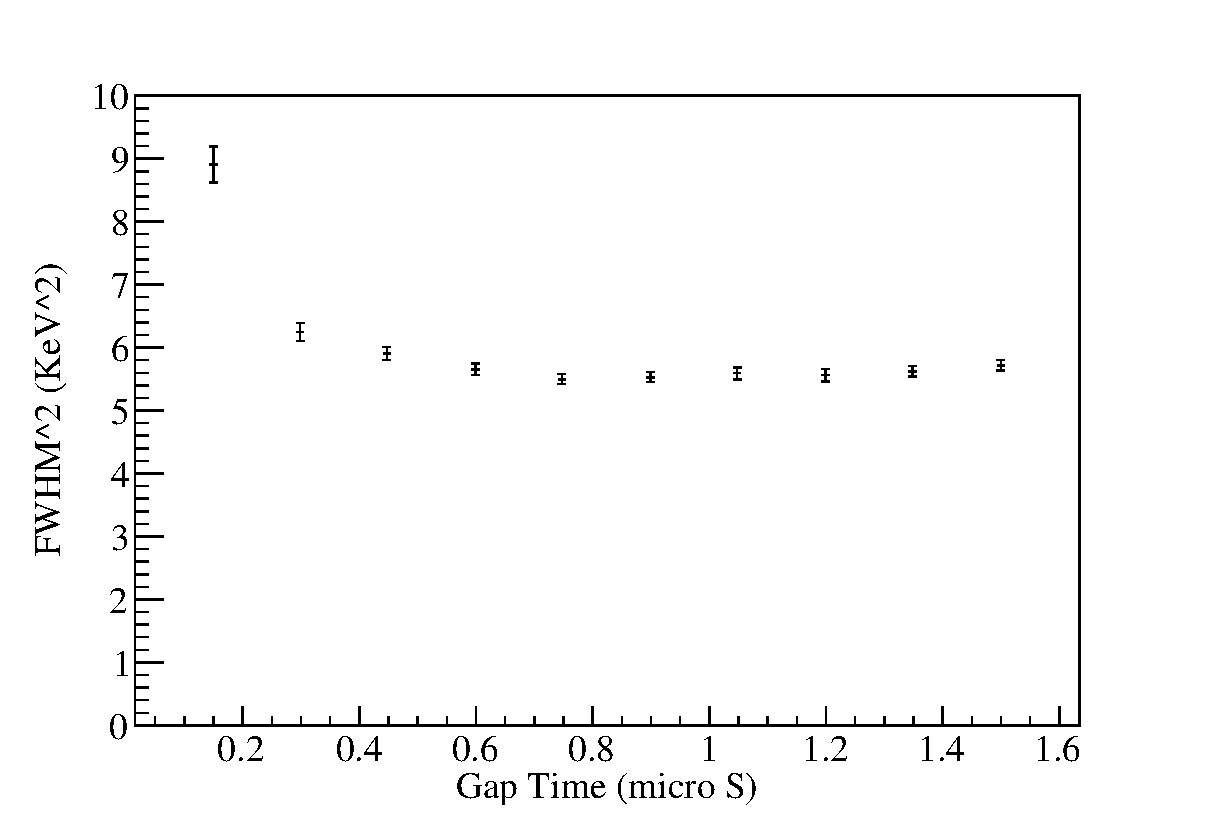
\includegraphics[width=.5\textwidth]{gap_min.eps}
\caption{The square of the FHWM of the $1.3 MeV\gamma$ vs gap time which was varied in $.15 \mu S$ increments. The error drops rapidly as the effect of ballistic deficit is overcome.  
\label{gap_min}}
\end{figure}


\begin{equation}
\label{gauss_lin}
F(E_{\gamma}) = e^{-\frac{1}{2}(\frac{E-E_{\gamma}}{\sigma})^2}+a\cdot x+b
\end{equation}


\noindent using the scipy non-linear least squares fitting routine. The FWHM of the results was taken as $2.35*\sigma$. Figure ~\ref{peak_fit} shows a representative fit using this method.  Plotting the square of these values vs the shaping time allows inference into the relative contributions to the systems electronic noise. The square of the series noise from the system varies as $\frac{C_1}{\tau}$, the square of the parallel noise varies as $C_2 \cdot \tau$, and the square of the $\frac{1}{f}$ noise is independent of the shaping time\cite{Radeka}. To determine these contributions, the FWHM obtained were plotted and fit using a $\chi^2$ minimization routine, FUMILI, with a function of the form;

\begin{equation}
\label{noisefunc}
\text{FWHM}(\tau) =  C_1 \cdot \tau + C_2 + \frac{C_3}{\tau}
\end{equation}


\noindent The results are shown in Figure ~\ref{shapemin}. The minimum value of this function, $8 \mu S$, was used for the remainder of the analysis. Since the electronic noise was not measured independently it was not possible to separate the $\frac{1}{f}$ noise contribution from the statistical uncertainty. Thus the $C_2$ fit parameter is representative of a combination of statistical and $\frac{1}{f}$ uncertainty.  The fit resulted in a poor minimum $\chi^2$ value suggesting that either there was other noise contributions which are not accounted for by this model, or the uncertainties provided from the parameter estimation routine were erroneously small.
\begin{figure}
\includegraphics[width=.52\textwidth]{balistic_deficit.eps}
\caption{Comparing the two pulses on the left, the top one has a longer rise time than the bottom. Looking at the shape of the trapezoid for the two pulses shows a slow trend up towards the full value for the peak with a longer rise time (top). The trapezoid corresponding to the shorter rise time (bottom) is flat across the range. By selecting a value near the end of the flat top the effect of ballistic deficit on spectral resolution can be mitigated. 
\label{balistic}}
\end{figure}

To optimize the gap time, a similar process was used. The shaping time was held constant and the gap time was incremented in $0.15\mu S$ increments. The Square of the resultant FWHM and associated errors are shown in Figure ~\ref{gap_min}. Errors were determined from parameter estimates and then propagated. The minimum value of $0.9\mu s$ was used for the remainder of the analysis. The effect on resolution at lower gap times can be in part attributed to ballistic deficit. This occurred due to differential charge collection times causing the exponential output signal to have a non negligible rise time. This deformed the shape of the trapezoid differentially for different rise times. By using a sufficiently long gap time and using a value near then late time edge, the filter can encounter the full peak before it returns towards zero minimizing this effect. Two shaped pulses with differing amounts of ballistic deficit are shown in Figure ~\ref{balistic} as an illustration of this phenomenon. A triangular filter (gap time = 0) was employed as a lower limit on this test and always provided worse resolution as there was no means of compensating for the ballistic deficit.




\begin{figure}[b]
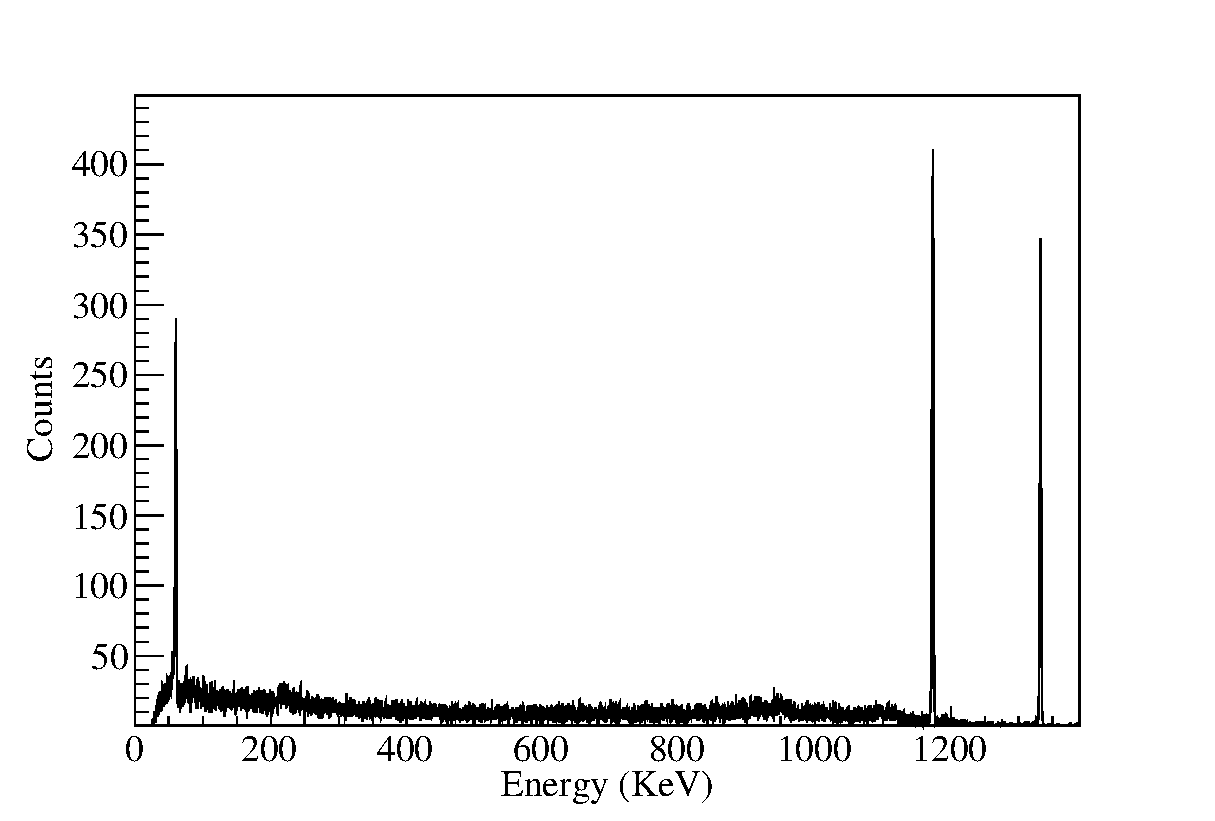
\includegraphics[width=.5\textwidth]{spectrum.eps}
\caption{The spectrum resulting from using optimized peaking and gap time for a data set where both $^{241}Am$ and $^{60}Co$ were present. 
\label{spectrum}}
\end{figure}




Finally, using these optimized parameters a spectrum,Figure ~\ref{spectrum}, was generated from a data set where both an $^{241}Am$ and $^{60}Co$ contributed to the spectra. To determine the resolution, the same fitting algorithm described above was applied to the three peaks. The results are summarized in table \ref{resolution}.

\begin{table}[h!]
\caption{The resolution resulting from optimized parameters for the digital system.  
\label{resolution}}
\centering
\begin{tabular}{ccc}
\hline
Energy (KeV) & FWHM (KeV) & Resolution (\%)   \\
 \hline
$59.45$ & $1.69 \pm 0.053$ & $2.8 \pm 9.0 \cdot 10^{-2}$ \\
$1173$ & $2.21 \pm 0.020$ &$ 0.19 \pm 1.9 \cdot 10^{-3}$ \\
$1332 $& $2.30 \pm 0.028$& $0.17 \pm 2.1\cdot 10^{-3}$ \\
\hline
\end{tabular}
\end{table}

\noindent Uncertainties quoted come from parameter error estimation which was then propagated as necessary. To determine the Fano Factor, the square of these values was plotted against energy. The result was fit via the FUMILI $\chi^2$ minimization routine using the following function relating the fano factor to the measured uncertainty and electronic noise
\begin{figure}[b]
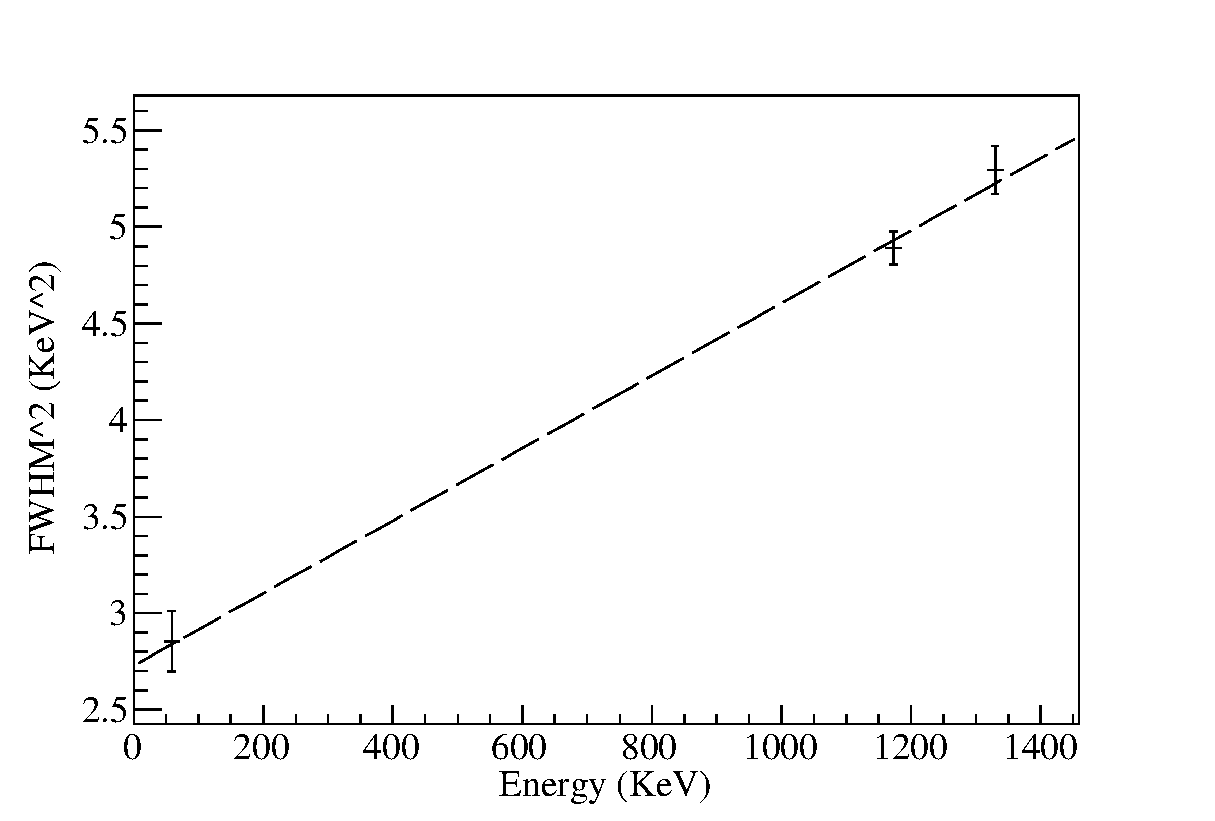
\includegraphics[width=.5\textwidth]{fano_factor_determination.eps}
\caption{The $\text{FWHM}^2$  plotted against the energy. The dashed line is the best fit to the expected model using $\chi^2$ minimization  
\label{fano}}
\end{figure}

\begin{equation}
\label{fano}
\delta E_{tot}^2 = 2.35^2 \cdot \epsilon E \cdot F+ \delta E_{e}^2
\end{equation} 
\noindent where $\delta E_{tot}^2$ is the FWHM obtained from curve fitting, $\epsilon$ is the energy required to produce an electron hole pair ($2.95 eV$), F is the fano factor, and $\delta E_{e}^2$ is the electronic noise contribution. This formula neglects the contribution from charge trapping. It also provided a means of determining the electronic noise contribution. Figure \ref{fano} shows the data points used and the fit obtained. This resulted in the following values:
\[
F = 0.115 \pm 0.009 \\
\]
\[and
\]
\[
\delta E_{e} = 1.65 \pm 0.05 \\ 
\]
The $\frac{\chi^2}{NDF}$ resulting from the fit was 0.7 suggesting slight overestimation of the uncertainties on the FWHM values. Considering uncertainty, this value is within the range expected for germanium, but it is slightly high. This is expected due to neglecting charge carrier trapping contributions to the total uncertainty. The agreement shows that this is a relatively small effect on the overall noise of the system.
To compare this with analog methods, the FWHM of a peak resulting from the described analog setup was minimized by varying the shaping time and correcting for pole zero each time. The results are summarized in table \ref{analog}. 

\begin{table}[h]
\caption{The resolution resulting from optimized parameters for the analog system and comparison to the digital system. 
\label{analog}}
\centering
\begin{tabular}{cccc}
\hline
Energy (KeV) & FWHM (KeV) & Resolution (\%)&$\frac{Analog}{Digital}$   \\
 \hline
$59.45$ & 1.01& $1.7$ & 0.60\\
$1173$ & 1.68 &$ 0.143 $ & 0.76\\
$1332 $& 1.97 & 0.147 & 0.86\\
\hline
\end{tabular}
\end{table}

Unfortunately at the time of collection the values from MAESTRO peak fitting routine were recorded without uncertainty, so no error is reported on these values. The analog system in this case produced better resolution. The digital system data were collected on had a strong electronic noise component somewhere on digital side of the system. No solution was found. 
\section{conclusion}
\label{conc}
In this lab the student familiarized himself the the digital acquisition system employing Struck SIS3302 waveform digitizers, explored digital filtering techniques, investigated sources of noise in acquisition system, and considered the general problem of detecting high energy gamma radiation. The use of modern fast adc's has revolutionized modern spectroscopy. This lab has provided a solid background in the important considerations for work done with these systems. The code developed in this experiment can be expanded to include more advanced applications. These include pile up rejection, pile up deconvolution, pulse shape discrimination, and temporal event determination.  


\begin{thebibliography}{99}

\bibitem{root}Rene Brun, Fons Rademakers, 
ROOT - An Object Oriented Data Analysis Framework
http://root.cern.ch/

\bibitem{jordanov_1} Valentin T. Jordanov, Glenn F. Knoll, Digital synthesis of pulse shapes in real time for high resolution radiation spectroscopy, Nuclear Instruments and Methods in Physics Research Section A: Accelerators, Spectrometers, Detectors and Associated Equipment, Volume 345, Issue 2, 15 June 1994, Pages 337-345, ISSN 0168-9002, 

\bibitem{knoll} G.F. Knoll, Radiation Detection and Measurement, (John Wiley \& Sons, 2000), 3rd Ed.

\bibitem{python}Fernando Pérez, Brian E. Granger, IPython: A System for Interactive Scientific Computing, Computing in Science and Engineering, vol. 9, no. 3, pp. 21-29, May/June 2007, doi:10.1109/MCSE.2007.53. URL: http://ipython.org

\bibitem{Radeka}V Radeka, Low-Noise Techniques in Detectors, Annual Review of Nuclear and Particle Science, Vol. 38: 217-277 (Volume publication date December 1988)






\end{thebibliography}

\end{document}
